%!TEX root = dissertation.tex

\chapter{Evaluación del método de evaluación (DBA) y del lenguaje para diseñar evaluaciones (SASQL)} \label{Ap:eval-metodo}

% the code below specifies where the figures are stored
\ifpdf
    \graphicspath{{Apendice/figures/PNG/}{Apendice/figures/PDF/}{Apendice/figures/}}
\else
    \graphicspath{{Apendice/figures/EPS/}{Apendice/figures/}}
\fi



\global\mdfdefinestyle{cuestionarioST}{%
linecolor=blue,linewidth=2pt,%
leftmargin=1cm,rightmargin=1cm
}

\global\mdfdefinestyle{hipotesis0}{%
linecolor=black,linewidth=1pt,%
leftmargin=1cm,rightmargin=1cm
}
Este apéndice contiene el cuestionario utilizado para la evaluación del método DBA y del lenguaje SASQL. Además, en un segundo apartado se analizan las respuestas recogidas. Las secciones de este apéndice son:

\begin{itemize}
	\item Cuestionario (ver sección~\ref{apc:eval:metodo:cuestionario})
	\item Resultados  (ver sección~\ref{apc:eval:metodo:resultados})
\end{itemize}

\newpage

\section{Cuestionario} \label{apc:eval:metodo:cuestionario}
	
	\subsection*{A. Sexo}

\begin{mdframed}[style=cuestionarioST]
			\begin{itemize}
				\item Hombre
				\item Mujer
			\end{itemize}
\end{mdframed}

	\subsection*{B. Rama}

\begin{mdframed}[style=cuestionarioST]
			\begin{itemize}
				\item Arte y humanidades
				\item Ciencias sociales y jurídicas
				\item Ciencias
				\item Ciencias de la salud
				\item Ingeniería y arquitectura
			\end{itemize}
\end{mdframed}

	
\newpage

	\subsection*{C. Cuestiones sobre el método DBA}

\begin{mdframed}[style=cuestionarioST]
	En este método, los docentes diseñan una evaluación de los estudiantes a partir de la información contenida en el registro del entorno virtual de aprendizaje y evalúan los resultados. El docente podrá aceptar y utilizar los resultados, descartarlos o redefinir una nueva evaluación para contrastar los resultados anteriores.
\end{mdframed}


	\paragraph*{C.1 ¿Considera el método DBA adecuado para obtener automáticamente indicadores de entornos de aprendizaje virtual?}

\begin{mdframed}[style=cuestionarioST]
			\begin{itemize}
				\item Sí
				\item No
				\item Ns/nc
			\end{itemize}
\end{mdframed}


	\paragraph*{C.2 ¿Cuál de las siguientes características considera que aporta el método DBA?}

Marque una opción para cada característica siendo (1) totalmente de acuerdo, (2) de acuerdo, (3) ni acuerdo ni en desacuerdo, (4) en desacuerdo y (5) totalmente en desacuerdo.

\begin{table}[H]
  \begin{center}
  \begin{tabular}{| m{5cm} | c | c | c | c | c |}
    \hline
    CARACTERISTICAS & (1) & (2) & (3) & (4) & (5) \\
    \hline
    \hline
    Objetividad &  &  & & & \\
    \hline
    Adaptabilidad &  &  & & & \\
    \hline
    Sistematicidad &  &  & & &  \\
    \hline
    Flexibilidad &  &  & & &  \\
    \hline
    Fiabilidad &  &  & & &  \\
    \hline
  \end{tabular}
\end{center}
\caption{Selección de características del método DBA}
\label{tab:ap:caracteristicas:metodo}
\end{table}

\newpage

\subsection*{D. Cuestiones sobre el lenguaje SASQL}

\begin{mdframed}[style=cuestionarioST]
	Con este lenguaje los docentes pueden diseñar evaluaciones a partir de la información contenida en el registro de aprendizaje virtual. 
\end{mdframed}

	\paragraph*{D.1 ¿Considera que el lenguaje presentado es útil para diseñar y contrastar estrategias de evaluación a partir de los registros de actividad de los entornos de aprendizaje virtual?}

\begin{mdframed}[style=cuestionarioST]
			\begin{itemize}
				\item Sí
				\item No
				\item Ns/Nc
			\end{itemize}
\end{mdframed}


	\paragraph*{D.2 ¿Cuáles de las siguientes características considera que aporta el lenguaje presentado?}

Marque una opción para cada característica siendo (1) totalmente de acuerdo, (2) de acuerdo, (3) ni acuerdo ni en desacuerdo, (4) en desacuerdo y (5) totalmente en desacuerdo.

\begin{table}[H]
  \begin{center}
  \begin{tabular}{| m{5cm} | c | c | c | c | c |}
    \hline
    CARACTERISTICAS & (1) & (2) & (3) & (4) & (5) \\
    \hline
    \hline
    Facilidad de aprendizaje &  &  & & & \\
    \hline
    Eficacia &  &  & & & \\
    \hline
    Ahorra tiempo &  & & & &  \\
    \hline
    Escalabilidad &  & & & &  \\
    \hline
    Capacidad de reutilización &  &  & & &  \\
    \hline
    Fiabilidad &  &  & & & \\
    \hline
  \end{tabular}
\end{center}
\caption{Selección de características del lenguaje SASQL}
\label{tab:ap:caracteristicas:sasql}
\end{table}

\newpage

	\paragraph*{D.3 Tomando como ejemplo la siguiente consulta del DSL, utilizada para obtener información de la interacción de los estudiantes en el foro del campus virtual:}

\begin{minted}[linenos,frame=lines,
               framesep=2mm]{pascal}
Evidence interaccion_foro:  
	get students 
	show interaction 
	in forum.
\end{minted}


\begin{mdframed}[style=cuestionarioST]
	¿Considera entendible la consultas del DSL?
			\begin{itemize}
				\item Sí
				\item No
				\item Ns/Nc
			\end{itemize}
\end{mdframed}


	\paragraph*{D.4 Tomando como ejemplo los resultados que se obtienen de la consulta anterior:}

\begin{figure}[H]
  \begin{center}
    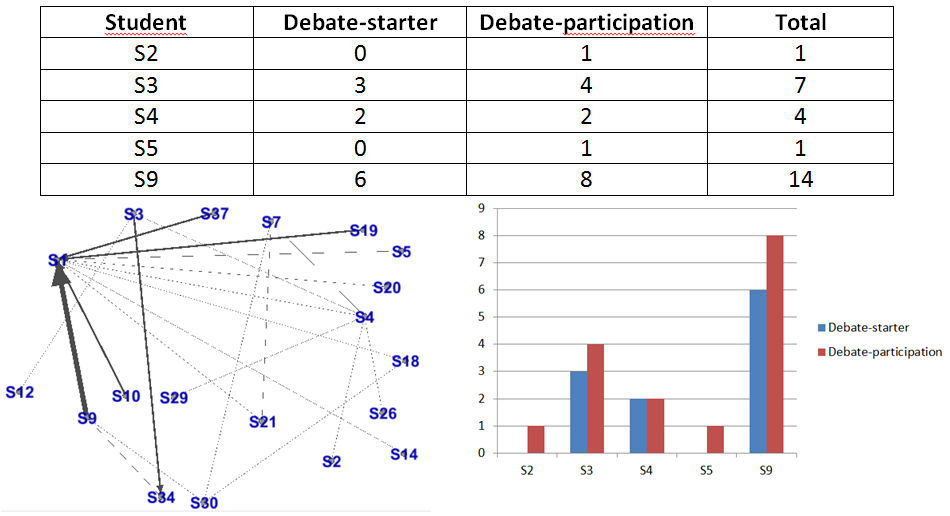
\includegraphics[scale=0.4]{ResultadosConsulta.png}
  \end{center}
  \caption{Resultados consulta}
  \label{fig:ape:resultados:consulta}
\end{figure}

\begin{mdframed}[style=cuestionarioST]
	¿Considera los resultados entendibles?
			\begin{itemize}
				\item Sí
				\item No
				\item Ns/Nc
			\end{itemize}
\end{mdframed}



\newpage

% RESULTADOS COPIADOS DEL OTRO.
\section{Resultados} \label{apc:eval:metodo:resultados}

En esta sección se muestran y analizan en detalle los resultados del cuestionario. %Los comentarios sobre los resultados de los profesores se muestran en el capítulo X (esto se dice en la tesis de la uoc, tendré que ver qué comento yo).

\subsection{Poblaciones}

En este cuestionario participaron docentes que asistieron a las Jornadas de Innovación Docente de la Universidad de Cádiz. Se realizó una presentación del método y la herramienta, y tras un turno de preguntas, se pasó el cuestionario mostrado en el apartado anterior.


% SEGUIR POR AQUI

\subsection{Participantes}

...
